\chapter{Magnetic vortex effects on first-order reversal curve (FORC) diagrams for greigite dispersions}
\label{ch:res-3}
\fancyhead[L]{Chapter 4. Single-vortex effects on FORC diagrams}
\fancyhead[C]{}
\fancyhead[R]{}
\fancyfoot[C]{\thepage}

This Chapter is submitted for publication as Valdez-Grijalva, M. A., Muxworthy, A. R., Williams, W., \'O Conbhu\'i, P., Nagy, L., Roberts, A. P., Heslop, D., 2018. Magnetic vortex effects on first-order reversal curve (FORC) diagrams for greigite dispersions. Earth Planet. Sci. Lett., in review.\par

M.\,V.\,G. designed the experiment, performed the simulations and wrote the article. W.\,W., P.\,C. and L.\,N. wrote the micromagnetic code. M.\,V.\,G., A.\,M., A.\,R. and D.\,H. analysed the results.\par

\section*{Abstract}
First-order reversal curve (FORC) diagrams are used increasingly in geophysics for magnetic domain state identification. The domain state of a magnetic particle is highly sensitive to particle size, so FORC diagrams provide a measure of magnetic particles size distributions. However, the FORC signal of particles with nonuniform magnetisations, which are the main carrier of natural remanent magnetisations in many systems, is still poorly understood. In this study, the properties of non-interacting, randomly oriented dispersions of greigite (Fe$_3$S$_4$) in the uniform single-domain (SD) to non-uniform single-vortex (SV) size range are investigated via micromagnetic calculations. Signals for SD particles ($<50\nm$) are found to be in excellent agreement with previous SD coherent-rotation studies. A transitional range from $\roughly$50$\nm$ to $\roughly$70$\nm$ is identified for which a mixture of SD and SV behaviour produces complex FORC diagrams. Particles $> \roughly 70\nm$ have purely SV behaviour with the remanent state for all particles in the ensemble represented by the vortex state. It is found that for SV ensembles the FORC diagram provides a map of vortex nucleation and annihilation fields and that the FORC distribution peak should not be interpreted simply as the coercivity of the sample, but as a vortex annihilation field on the path to saturation.\par

\section{Introduction}
First-order reversal curve (FORC) diagrams are a powerful tool in rock magnetic studies, which allow mineral and domain state identification as well as quantification of magnetostatic interactions among particles \citep{Pike1999,Roberts2000,Roberts2014,Dumas2007,Egli2010}. As such, they have been the subject of numerical studies aimed at relating the behaviour of individual magnetic particles and small assemblages to experimental bulk properties \citep{Pike1999,Carvallo2003,Carvallo2006,Muxworthy2004,Muxworthy2005,Newell2005,Harrison2014,ValdezGrijalva2017,Roberts2017}.\par

With the exceptions of \citet{Carvallo2003} and \citet{Roberts2017}, all of these numerical studies have concentrated on FORC diagrams for ideal, uniformly magnetised single-domain (SD) particles. They have shown that uniaxial SD particles produce patterns in FORC diagrams \citep{Muxworthy2004,Newell2005,Harrison2014}, that are distinct from those for SD materials with cubic anisotropy \citep{Muxworthy2004,Harrison2014,ValdezGrijalva2017}. However, it is well-documented that most natural systems have magnetic signals dominated by larger grains with more complex magnetic domain states \citep{Dunlop,Roberts2017}. Grains just above the SD threshold size (e.g., $\roughly 64 \nm$ for equidimensional magnetite, $\roughly 54 \nm$ for greigite), are typically in a single-vortex (SV) state. The SV state dominates magnetic structures over an order of magnitude of size variations \citep{Nagy2017, ValdezGrijalva2017B}, which is much wider than the stable SD size range. SV grains have recently been found to be geologically meta-stable and retain relatively high remanences \citep{Almeida2014,Nagy2017, ValdezGrijalva2017B}.\par

Previous experimental studies on nano-patterned arrays of SV particles \citep{Pike1999B,Dumas2007} found that FORC diagrams are significatively more complex than for SD signals, with complex off-axis ``butterfly'' patterns that are related to vortex nucleation/annihilation processes. However, it is difficult to relate the behaviour of 2D nano-patterned arrays to the behaviour of natural particle systems found in geological samples. In natural samples, particles with varying size and orientation are dispersed in 3 dimensions. Thus, it is important to understand the contribution of dispersions of randomly aligned SV particles to FORC diagrams. Numerical modelling can aid the study of such systems. \citet{Carvallo2003} used a finite-difference model to calculate the FORC distributions of SV magnetite particles; however, that study primarily examined the effects of interactions between small clusters of cubic grains, and neither random particle distributions nor realistc grain morphologies were included.\par

In this study, we employ a micromagnetic finite element method (FEM) to obtain FORC diagrams for non-interacting ensembles of SD and SV greigite (Fe$_3$S$_4$). Greigite is the iron-sulphide counterpart to magnetite. Recent interest in greigite comes from both its promising properties for material science \citep{Li2014} and the abundance of this mineral in sedimentary rocks for Earth science \citep{Roberts2011}. FORC diagrams are often used to help identify greigite. The relatively high anisotropy of greigite means that the behaviour of this mineral is representative of cubic-anisotropic ferri- and ferro- magnets like magnetite and iron. We calculate FORC diagrams for simulations of non-interacting dispersions of randomly oriented greigite with sizes 30--80$\nm$; this size range covers the SD--SV threshold \citep{ValdezGrijalva2017B}. Simulations are carried out on an ensemble of 500 particles with random orientations. The unstructured discretisation of FEMs allows us to study realistic greigite particle shapes as observed in nature. We determine the onset of SV behaviour and its consequences for FORC diagram interpretation.\par
%-----------------------------------------------------

\section{Methods}
\subsection{The micromagnetic algorithm}\label{mmsection2}
%A ferromagnetic material{\textemdash}neglecting thermal and magnetostrictive effects{\textemdash}has a Gibbs free-energy functional given by \citep{Brown}:
%\begin{equation}
%E_\text{G} = \int_{\Omega} (\phi_{\text{exchange}} + \phi_{\text{anisotropy}} + \phi_{\text{stray}} + \phi_{\text{external}})\,\text{d}^3 \boldsymbol{r},
%\end{equation}
%where $\Omega$ is the ferromagnetic volume. Here,
%\begin{equation}
%\phi_{\text{exchange}}=A|\nabla\boldsymbol{m}|^2,
%\end{equation}
%where $\boldsymbol{m}$ is the reduced magnetisation vector and $A$ the exchange stiffness constant, provides an expression for the energy density due to quantum-mechanical exchange forces \citep{Landau1935}.\par
%\begin{equation}
%\phi_{\text{anisotropy}}=\frac{K_1}{2}\sum_{i\neq j}\gamma_i^2\gamma_j^2 + K_2\prod_i\gamma_i^2,
%\end{equation}
%where $\gamma_i$ represent the direction cosines and $K_1$ and $K_2$ the first and second magnetocrystalline anisotropy (MCA) constants, is the MCA energy density in the cubic anisotropy system. In terms of the reduced magnetisation vector components, this becomes:
%\begin{equation}
%\phi_{\text{anisotropy}}=K_1(m_x^2m_y^2+m_y^2m_z^2+m_z^2m_x^2),
%\end{equation}
%where $K_2$ is neglected because $K_1$ is the dominant term at room temperature. The magnetostatic self-energy density is given by:
%\begin{equation}
%\phi_{\text{stray}}=-\frac{\mu_0M_\text{S}}{2}\boldsymbol{m}\cdot\boldsymbol{H}_{\text{stray}},
%\end{equation}
%where $\boldsymbol{H}_{\text{stray}}$ is the stray field produced by the ferromagnetic body and $M_\text{S}$ is the saturation magnetisation. Finally, the energy density due to an external magnetic field $\boldsymbol{H}_{\text{external}}$ is:
%\begin{equation}
%\phi_{\text{external}}=-\mu_0M_\text{S}\boldsymbol{m}\cdot\boldsymbol{H}_{\text{external}}.
%\end{equation}\par

%Such magnetic particle systems will be driven spontaneously toward an equilibrium state with a locally minimal magnetic Gibbs free-energy \citep{Brown}. In this study we utilise a modified gradient descent method to find the equilibrium magnetisation \citep{OConbhui2017}.\par

A numerical micromagnetic FEM \citep{OConbhui2017} has been implemented to study the FORC properties of truncated octahedral greigite particles in the SD--SV size range. For details on the micromagnetic method see Section \ref{mmsection}.\par

The magnetic parameters of greigite used in this investigation are: the saturation magnetisation $M_\text{S}= 2.7 \times 10^5\,\text{A/m}$ \citep{Li2014}; the exchange stiffness constant $A=2\times10^{-12}\,\text{J}/\text{m}$ \citep{Chang2008}; and the first MCA constant $K_1=-1.7\times10^4\,\text{J}/\text{m}^3$ \citep{Winklhofer2014}. This set of parameters has been used in recent numerical studies of greigite \citep{ValdezGrijalva2017B,ValdezGrijalva2017}.\par

\subsection{The FORC model}
FORC diagrams are constructed from a class of partial hysteresis curves called first-order reversal curves \citep{Mayergoyz1986}, each starting at a value $B_a$ of the applied field along the main hysteresis branch and tracing the magnetisation as the field $B_b$ is increased to saturation. A magnetisation function on two variables $M=M(B_a, B_b)$ is thus obtained. The FORC distribution $\rho$ is then defined as \citep{Roberts2000}:
{\par\nobreak\noindent}
\begin{equation}
\rho=-\frac{1}{2}\frac{\partial^2 M}{\partial H_a \partial H_b}=-\frac{\mu_0^2}{2}\frac{\partial^2 M}{\partial B_a \partial B_b},
\end{equation}
where $\mu_0$ is the magnetic constant (or vacuum permeability) and $H=B/\mu_0$.\par

Once $M(B_a, B_b)$ is obtained, calculation of $\rho(B_a, B_b)$ is done by least-squares fitting of a degree 2 polynomial surface $a_0 + a_1 B_a + a_2 B_b + a_3 B_a B_b + a_4 B_a^2 + a_5 B_b^2 + \text{error} = M(B_a,B_b)$ on a subgrid of $M(B_a, B_b)$ centered around $(B_a, B_b)$ as determined by the so-called smoothing factor (SF) and including (2$\times$SF + 1)$^2$ points; the value of $\rho$ is then simply $-\mu_0^2 a_3/2$ \citep{Pike1999}. FORC diagrams are usually presented with rotated axes $B_c=(B_b - B_a)/2$, $B_u=(B_b + B_a)/2$.\par

Distributions with random orientation of magnetic particles with respect to the applied field were determined by taking 500 field orientations from a sector of the unit sphere (Fig. \ref{FIG_C4_01}). We use 500 field orientations as a workable compromise between accuracy and calculation speed. Also, for each particle/field-orientation, the hysteresis curve consists mostly of reversible motion of the magnetisation; thus, we only need to calculate the main branch of the hysteresis loop and the few reversal curves starting at the different switching fields along the main branch \citep{ValdezGrijalva2017}. The switching events are identified either by an abrupt change in the scalar net magnetisation $\Delta (M/M_\text{S})>0.1$ or a rotation of the net magnetisation vector larger than 5 degrees. These simplifications reduce vastly the number of calculations needed without loss of important information. The external-field rate of change for all models was 1$\mT$ with a saturation field of 250$\mT$, so that 501 reversal curves were calculated for each particle/field-orientation.
\begin{figure}
\centering
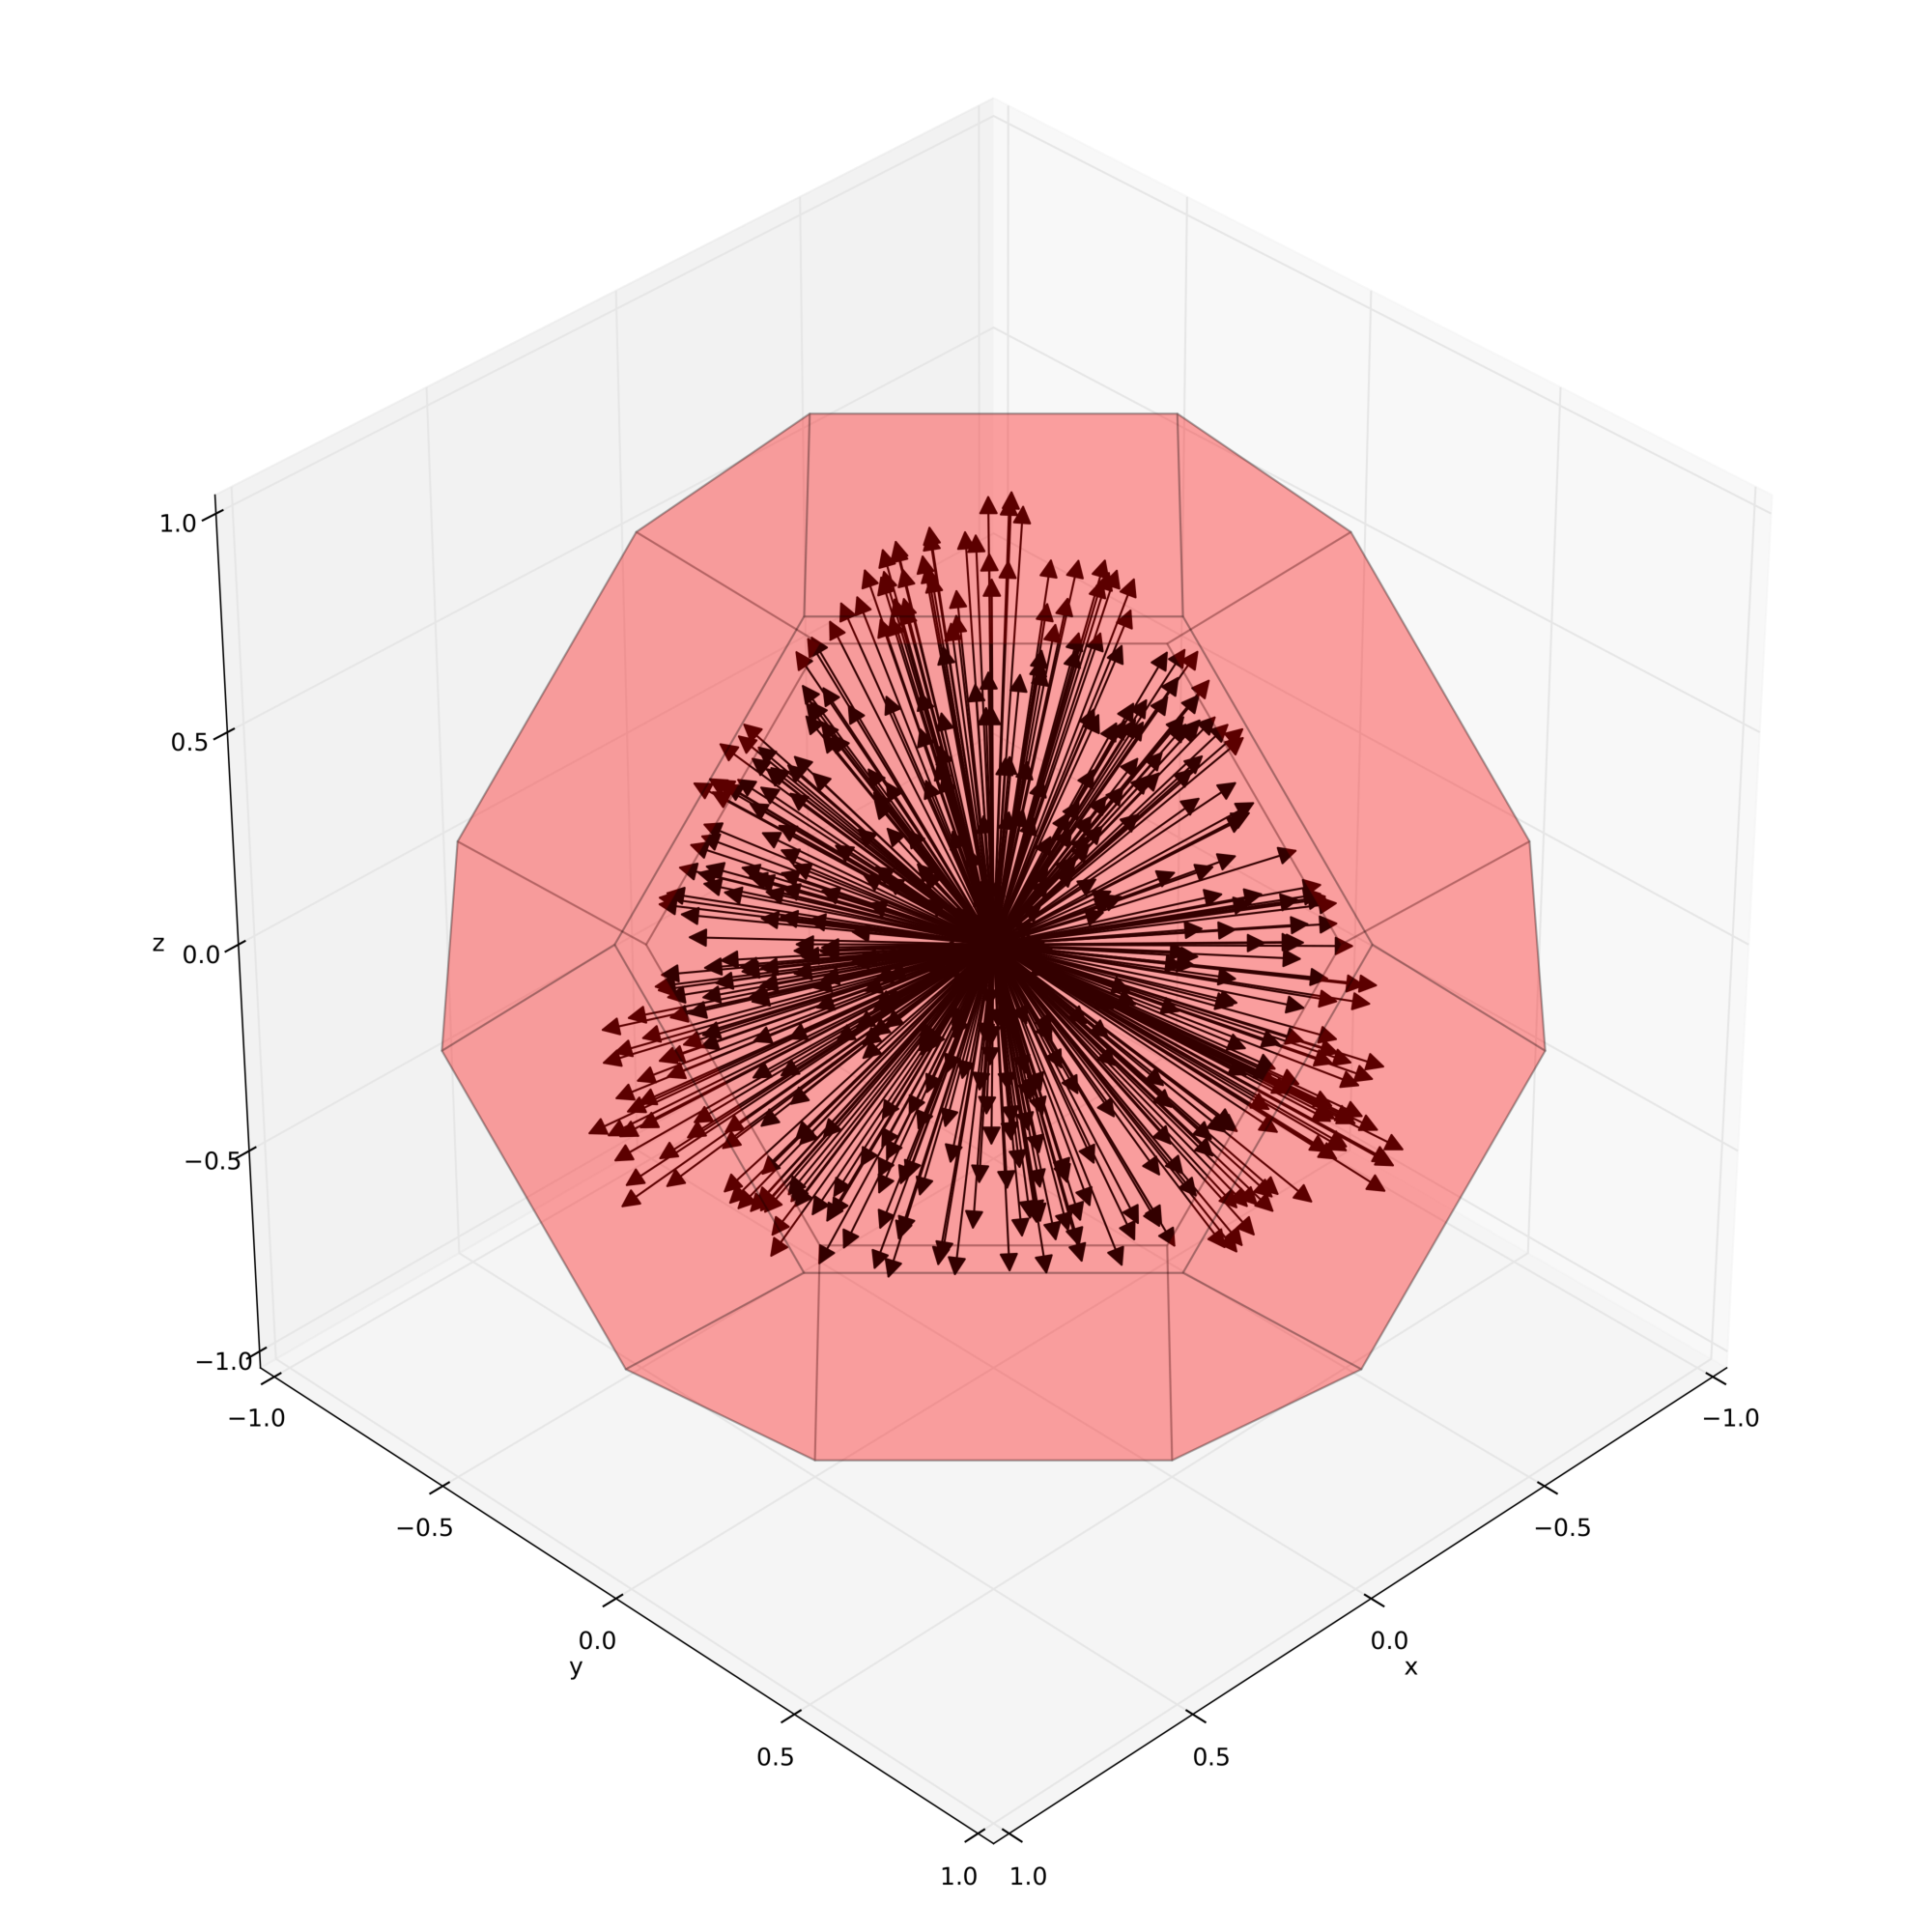
\includegraphics[width=\textwidth]{research-3/figs/FIG_01.pdf}
\caption[Model geometry and field orientations]{Model geometry and field orientations. The most common morphology for authigenic greigite is truncated octahedral. To avoid the high density of field orientations necessary near the sphere poles when using a regular grid, 500 random field orientations (arrows) were chosen from a uniform distribution over a sector of the unit sphere. The periodicity of the magnetocrystalline anisotropy and particle symmetry allow modelling of the effects of field orientations on only a sector of the sphere without loss of generality.}
\label{FIG_C4_01}
\end{figure}\par

Scanning electron and transmission electron micrographs of naturally occurring greigite samples \citep{Snowball1997,Vasiliev2008,Roberts2015} reveal that greigite tends to grow authigenically as well-defined regular truncated octahedral particles. Micromagnetic calculations for truncated octahedral greigite particles indicate that the SD--SV threshold occurs at $\roughly 54\nm$ \citep{ValdezGrijalva2017B}. In this study we model FORC diagrams for non-interacting ensembles of truncated octahedral greigite particles sized 30--80$\nm$ (where size is normalised to the volume of a cube) at 2$\nm$ size intervales. This range is chosen because it spans the transition from SD to SV behaviour.\par

%-----------------------------------------------------

\section{Results}
For ensembles with SD particles $<50\nm$, hysteresis behaviour is dominated by coherent rotation (Fig. \ref{FIG_C4_02}). This is seen by comparing FORC diagrams for these ensembles (Fig. \ref{FIG_C4_02}b) with those of idealised SD (effectively a single magnetic dipole), coherently rotating greigite particles (Fig. \ref{FIG_C4_02}a) determined using the method outlined in \citet{ValdezGrijalva2017}. Diagrams for particles $<50\nm$ obtained with the micromagnetic algorithm (Fig. \ref{FIG_C4_02}b) are offset $\roughly 3\mT$ to the left compared to the dipole model (Fig. \ref{FIG_C4_02}a); lower coercivities due to the micromagnetic algorithm, which includes flowering (small deviations from a perfect SD structure) as a result of magnetostatic self-interaction effects, account for this effect.
\begin{figure}
\centering
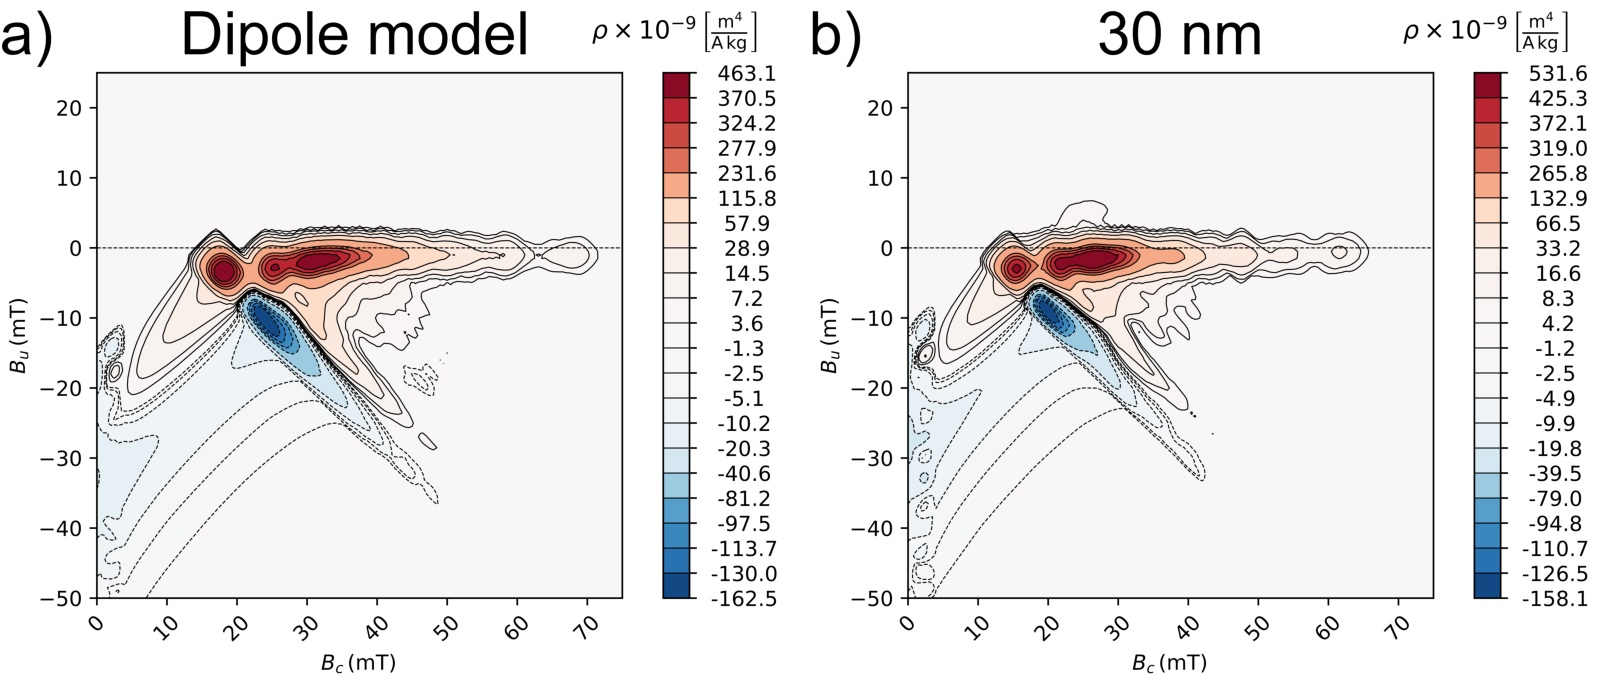
\includegraphics[width=\textwidth]{research-3/figs/FIG_02.pdf}
\caption[Comparison between dipole and micromagnetic model]{Comparison between FORC diagrams produced with dipole and micromagnetic models. a) Dipole model; FORC diagram (SF=4) for a non-interacting ensemble of idealised (size-independent) SD greigite particles obtained using the model of \citet{ValdezGrijalva2017}. b) Micromagnetic model; FORC diagram (SF=4) for a non-interacting ensemble of 30$\nm$ truncated octahedral greigite particles. Up to 48$\nm$, the FORC diagram is that of an ensemble of coherently rotating SD moments. For particles larger than 48$\nm$, magnetic vortex effects become important. Dashed contour lines denote negative $\rho$ values.}
\label{FIG_C4_02}
\end{figure}\par

Particles with cubic anisotropy have hysteresis behaviour that departs from that observed from the simple hysteron consisting of one plus and one minus magnetisation states. There exist intermediate easy axis states along hysteresis curves for the SD state \citep{ValdezGrijalva2017}. The tilted, elongated, negative-valued ridge (Fig. \ref{FIG_C4_02}) is a consequence of the availability of multiple hysteresis main branches caused by the cubic anisotropy. This negative-valued ridge is produced by the fraction of particles with a hard axis aligned closely with the applied field. These particles have the lowest switching fields: from the plus-state to an intermediate state at $B= B^{+}_{*}$ and from the intermediate state to the minus-state at $B=B^{*}_{-}$. Reversal curves with $B^{*}_{-} < B_a < B^{+}_{*}$ experience a sharp upward discontinuity at $B_b = B^{*}_{+} \leq |B^{+}_{*}|$ when hard-aligned particles return to the plus-state from their intermediate states. The combination of this type of irreversible event in hard-aligned particles causes the local peak at $B_c\approx 15 \mT, B_u\approx {-}3\mT$ (Fig. \ref{FIG_C4_02}b). For reversal curves with $B_a < B^{*}_{-}$, hard-aligned particles are initially in the minus-state and undergo irreversible rotation to an intermediate state on the path to positive saturation at $B=B^{-}_{*} = |B^{+}_{*}|$ due to the symmetry of the particles and the lack of magnetostatic interactions. The combination of these irreversible events causes a negative FORC distribution response at $B_a=B^{*}_{-}, B_b=B^{*}_{+}$. The sum effect of this type of response for many particles with a distribution of switching fields produces the elongated negative contribution observed in all SD ensembles, roughly along the line segment connecting ($B_c=18\mT,B_u=-6\mT$) with ($B_c=42\mT,B_u=-30\mT$).\par

The fraction of particles with easy axis alignment close to the applied field orientation exhibits hysteron-like behaviour, i.e., just two switching fields: from the plus-state to the minus-state $B^{+}_{-}$ and \textit{vice versa} $B^{-}_{+}$. The lack of interactions and the symmetry of particles in our simulations ensure that $|B^{+}_{-}| = B^{+}_{-}$. Thus, this fraction of particles produces FORC distribution responses at $B_a=B^{+}_{-}, B_b=B^{-}_{+}$. These types of irreversible responses accumulate on the line $B_a=-B_b$; they account for the most drastic changes in the magnetisation of the ensemble and, thus, account for the high slopes around the coercive field of the sample. This makes the position of the FORC diagram peak coincide with the coercivity of $B_\text{C}\approx 24\mT$ for SD ensembles.\par

Particles with size $d \geq 50\nm$ switch incoherently; that is, the FORC diagrams depart from coherent rotation behaviour associated with SD particles as the tight boomerang-shaped FORC diagram pattern exhibited by the SD greigite (Fig. \ref{FIG_C4_02}) becomes more fragmented (Fig. \ref{FIG_C4_03}). This change is driven initially by particles with hard axes close to the applied field nucleating hard-aligned vortices \citep{ValdezGrijalva2017B} as intermediate meta-stable states during hysteresis. Even though nucleation of hard-aligned vortices occurs in particles below the zero-field SD--SV threshold $d_0\approx 54\nm$ \citep{ValdezGrijalva2017B}, this is expected because vortex  nucleation greatly reduces the magnetic free-energy. A corollary of this is that a fraction of particles (with easy axis alignment close to the applied field) above the zero-field SD--SV threshold can remain in a SD state throughout hysteresis. These effects are due to distortion of the zero-field energy landscape by the applied field.
\begin{figure}
\centering
\includegraphics[width=\textwidth]{research-3/figs/FIG_03.pdf}
\caption[FORC diagrams with increasing vortex effects]{FORC diagrams with increasing vortex effects. SF=4 for all diagrams. a) 50$\nm$; b) 60$\nm$; c) 66$\nm$; and d) 76$\nm$. At these sizes, an ever larger fraction of the particle moments begin to switch with nonuniform magnetisations, i.e., vortex nucleation. At 76$\nm$ all particles are in the single vortex remanent state. Dashed contour lines denote negative $\rho$ values.}
\label{FIG_C4_03}
\end{figure}\par

An appreciable positive source in the FORC distribution appears along the $B_u=0$ axis at $B_c\approx 52\mT$ (the $B_c$ axis is not to be confused with the coercivity $B_\text{C}$) for ensembles with particles $\geq 54\nm$ (Fig. \ref{FIG_C4_04}, region 5); this contribution represents the annihilation of vortex states on the return to positive saturation. The elongated, negative ridge due to SD particles with cubic MCA and its corresponding symmetric positive response move to lower $(B_c, B_u)$ values (Fig. \ref{FIG_C4_04}, regions 1, 3) and the first responses for $B_u > 0$ begin to form (Fig. \ref{FIG_C4_04}, region 2); these are elongated features at 45$^{\circ}$ to the $B_u=0$ axis, which are different to the vertical widening usually attributed to magnetostatic interactions \citep{Pike1999,Muxworthy2004,Muxworthy2005}.
\begin{figure}
\centering
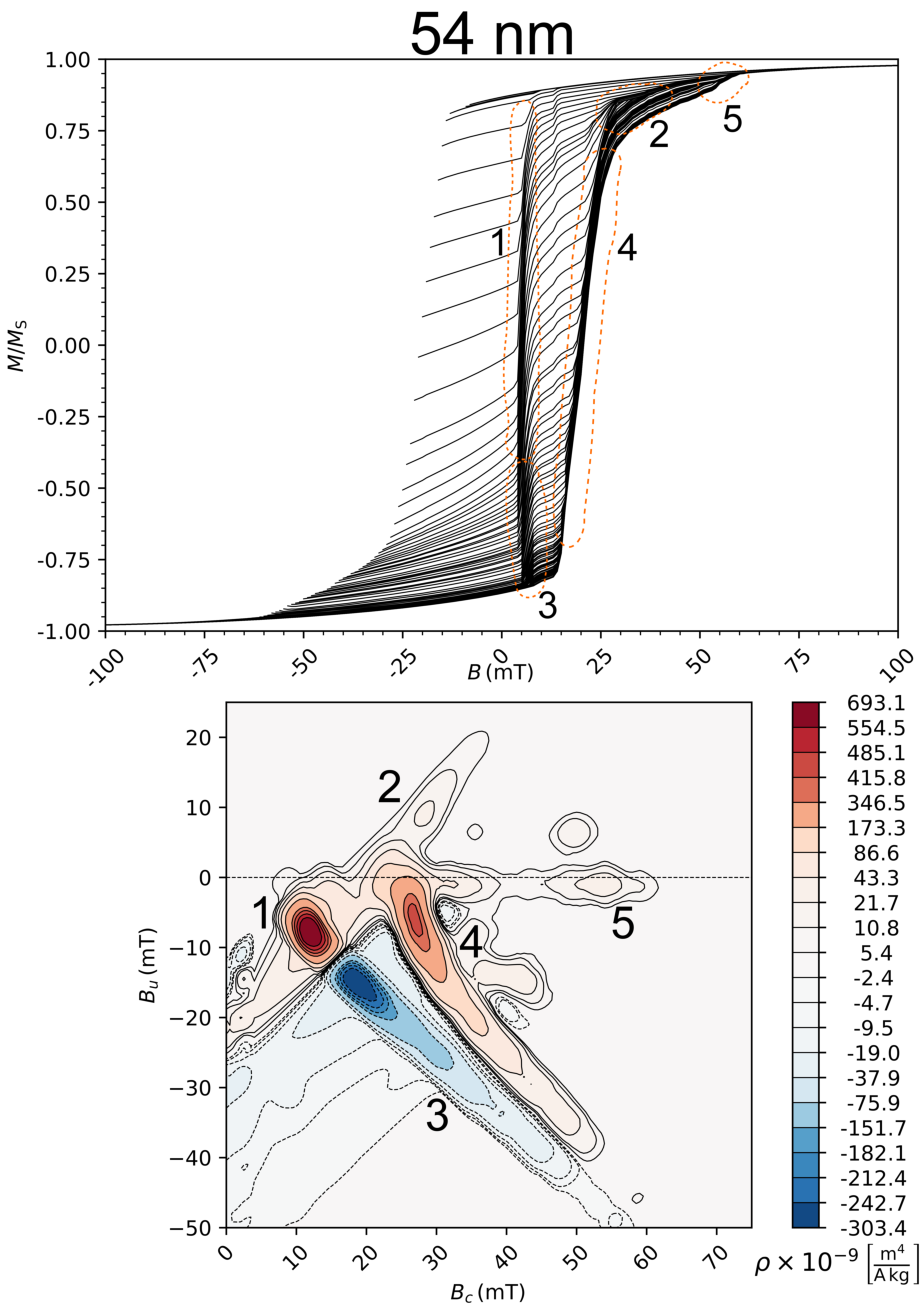
\includegraphics[width=0.9\textwidth]{research-3/figs/FIG_04.pdf}
\caption[FORC diagram and hysteresis curves of 54$\nm$-sized particles]{FORC diagram (SF=4) (bottom) and hysteresis curves (top) for 54$\nm$ particles. Annotations link the FORC diagram responses to the raw hysteresis curves. See text for details. Dashed contour lines on the FORC diagram denote negative $\rho$ values.}
\label{FIG_C4_04}
\end{figure}\par

For particles slightly below and above the SD--SV threshold $d_0$, vortex nucleation occurs only for negative applied field values, thus noticeable changes in the FORC diagrams (Fig. \ref{FIG_C4_03}a--c) are not evident in changes in the saturation remanence $M_\text{RS}$ to saturation magnetisation $M_\text{S}$ ratio up to 72$\nm$, whereas coercivity decreases sharply above 48$\nm$ (Fig. \ref{FIG_C4_05}b). The monotonically-decreasing coercivity trend is preserved up to 62$\nm$ when it rises from $B_{\text{C}}\approx 15 \mT$ to $\roughly 20 \mT$ for $d=68\nm$. With increasing size, coercivitiy decreases further, accompanied by a sharp decrease in $M_\text{RS}$ (Fig. \ref{FIG_C4_05}b). The drop in $M_\text{RS}$ is driven by particles nucleating vortices at $B_a>0$ for $d \geq 68\nm$. For $d \geq 76\nm$, all particles nucleate vortices so that the vortex state becomes the remanent magnetic domain state; this is reflected in the Day plot \citep{Day1977}, a scatter plot of the $M_\text{RS}/M_\text{S}$ ratio against the coercivity of remanence $B_\text{CR}$ (the field necessary to reduce the remanence to zero) to $B_\text{C}$ ratio, by particles 76$\nm$ and larger (Fig. \ref{FIG_C4_05}a), associated here with the SV state.
\begin{figure}
\centering
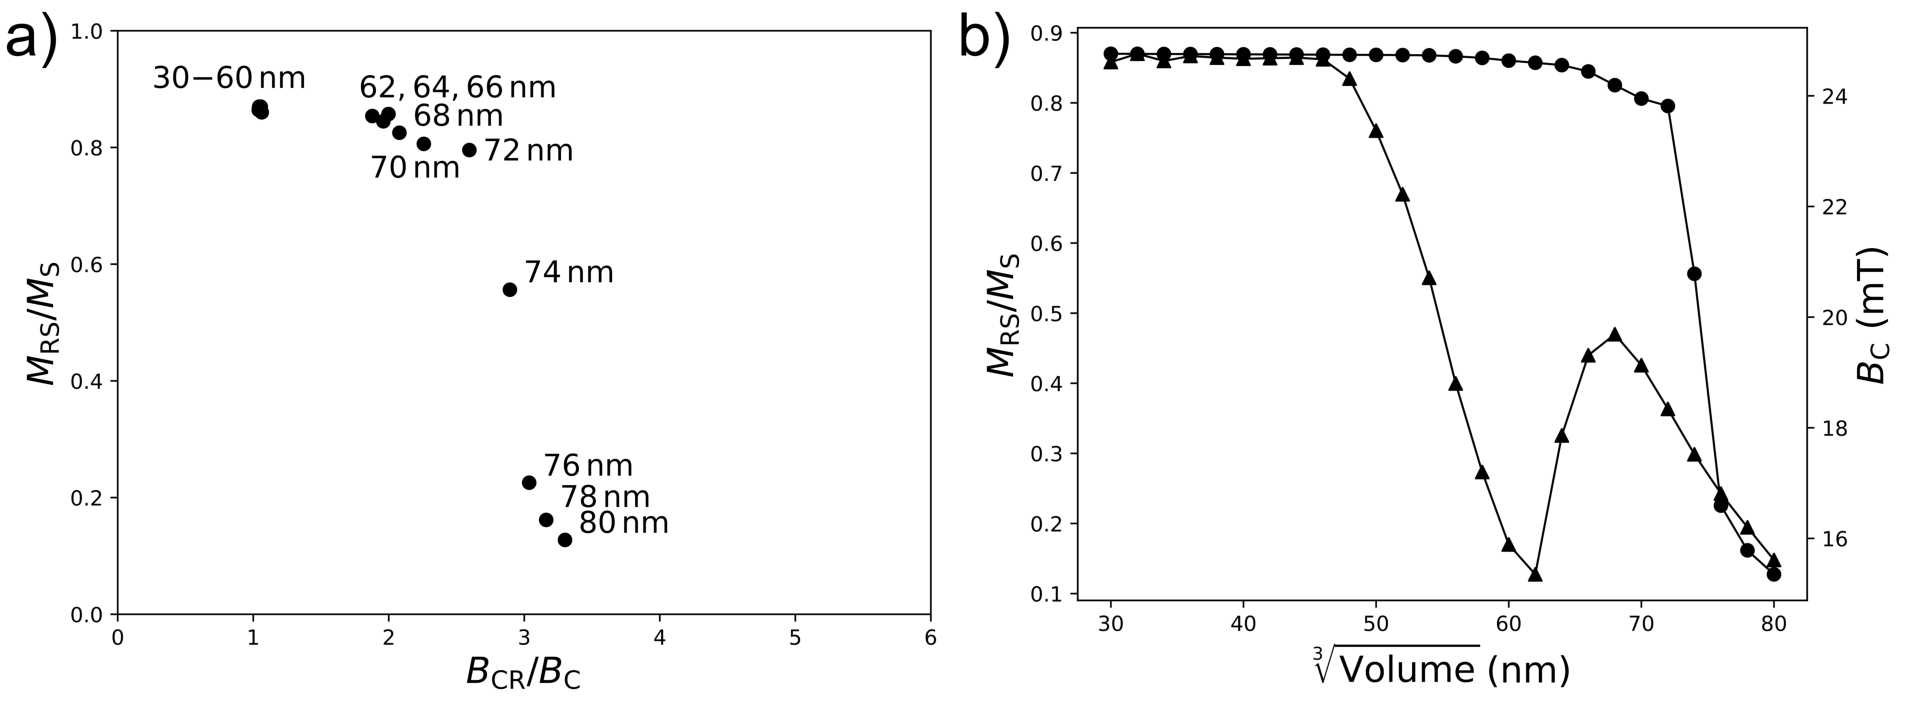
\includegraphics[width=\textwidth]{research-3/figs/FIG_05.pdf}
\caption[Day plot and remanence/coercivity against size]{Day plot and $M_\text{RS}/M_\text{S}$ and coercivity against particle size. a) The Day plot \citep{Day1977} contains data for SD particles up to 60$\nm$; however, we know from the micromagnetic solutions that vortices form from 50$\nm$ onward. Particles with size from 62 to 72$\nm$ plot in an unexpected region. Particles larger than 74$\nm$ plot with lower $M_\text{RS}/M_\text{S}$ and higher $B_\text{CR}/B_\text{C}$ values. b) Remanence (circles) and coercivity (triangles) versus particle size.}
\label{FIG_C4_05}
\end{figure}\par

Particles sized 62--72$\nm$ move away from the top left of the Day plot (Fig. \ref{FIG_C4_05}a) to a region with high remanence but larger $B_{\text{CR}}/B_{\text{C}}$ values. These sizes coincide with the anomalous coercivity increase for these sizes (Fig. \ref{FIG_C4_05}b). The increased coercivities can be explained by vortex nucleation, which causes hysteresis loops to become increasingly wasp-waisted (Fig. \ref{FIG_C4_06}) so that they cross the zero-magnetisation axis at increasing (absolute) values of the applied field strength. FORC diagrams for these sizes are the most complex of all those simulated here, and have a variety of features (Figs. \ref{FIG_C4_03}c, \ref{FIG_C4_06}) caused by the complex interplay of SV and SD effects. The elongated, negative ridge becomes more faint with increasing particle size, whereas the positive responses for $B_u>0$ become larger and move toward the $B_c=0$ axis with increasing size. Large, positive FORC responses for $B_u>0$ along the $B_c=0$ axis are expected for larger multi-domain (MD) grains \citep{Pike2001,Roberts2006}. The non-interacting nature of these ensembles means that the SD and SV FORC signals are linearly additive. Therefore, it is possible to discern the FORC responses due to SD (Fig. \ref{FIG_C4_06}, regions 3, 6) and SV particles (Fig. \ref{FIG_C4_06}, regions 1, 2, 4, 5, 7, 8).
\begin{figure}
\centering
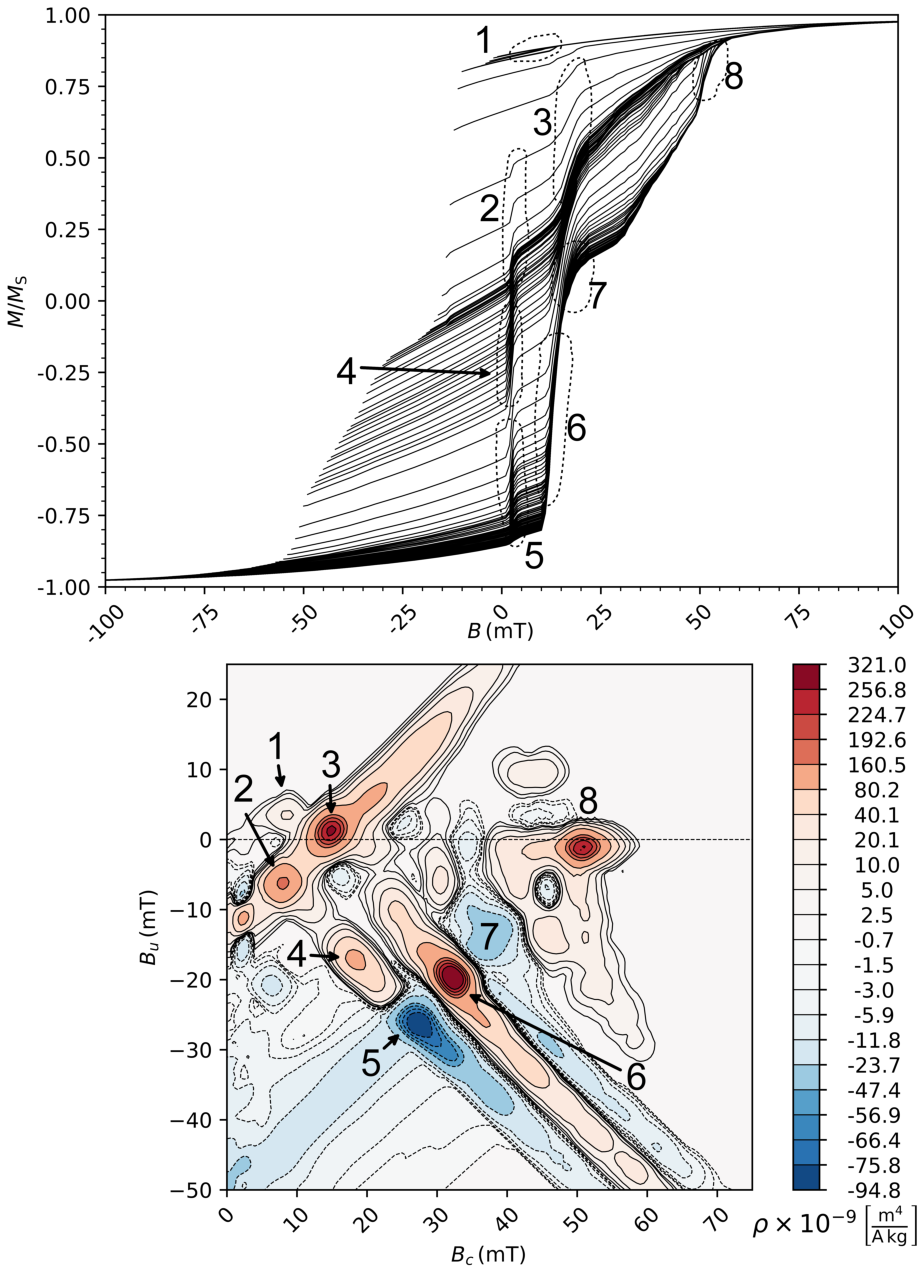
\includegraphics[width=0.9\textwidth]{research-3/figs/FIG_06.pdf}
\caption[FORC diagram and hysteresis curves of 62$\nm$-sized particles]{FORC diagram (SF=4) (bottom) and hysteresis curves (top) for 62$\nm$ particles. Annotations link the FORC diagram responses to the raw hysteresis curves. See text for details. Dashed contour lines on the FORC diagram denote negative $\rho$ values.}
\label{FIG_C4_06}
\end{figure}\par

The elongated, negative ridge typical of SD particles with cubic MCA \citep{ValdezGrijalva2017} disappears for particles $\geq 76 \nm$ (Fig. \ref{FIG_C4_03}d). A circular, negative feature centered roughly at ($B_c=8 \mT, B_u={-}8\mT$) becomes larger and of a magnitude comparable to the largest positive reponses. For $d=76$ and 78$\nm$ the negative response has a larger absolute value than the distribution peak (Fig. \ref{FIG_C4_03}d). For the 80$\nm$ particle model, a faint negative response appears centered roughly at ($B_c=40 \mT, B_u={-}12\mT$) (Fig. \ref{FIG_C4_07}, region 6). Fig. \ref{FIG_C4_07} represents the contribution of purely SV particles, that is, ensembles of particles that are all in a SV remanent state. It is logical that this FORC diagram is somewhat less complex than those for ensembles with a fraction of particles still in the SD state as well as some in the SV state; the difference is due to the field angle relative to particle orientation, as has also been shown by \citet{Roberts2017} for magnetite.
\begin{figure}
\centering
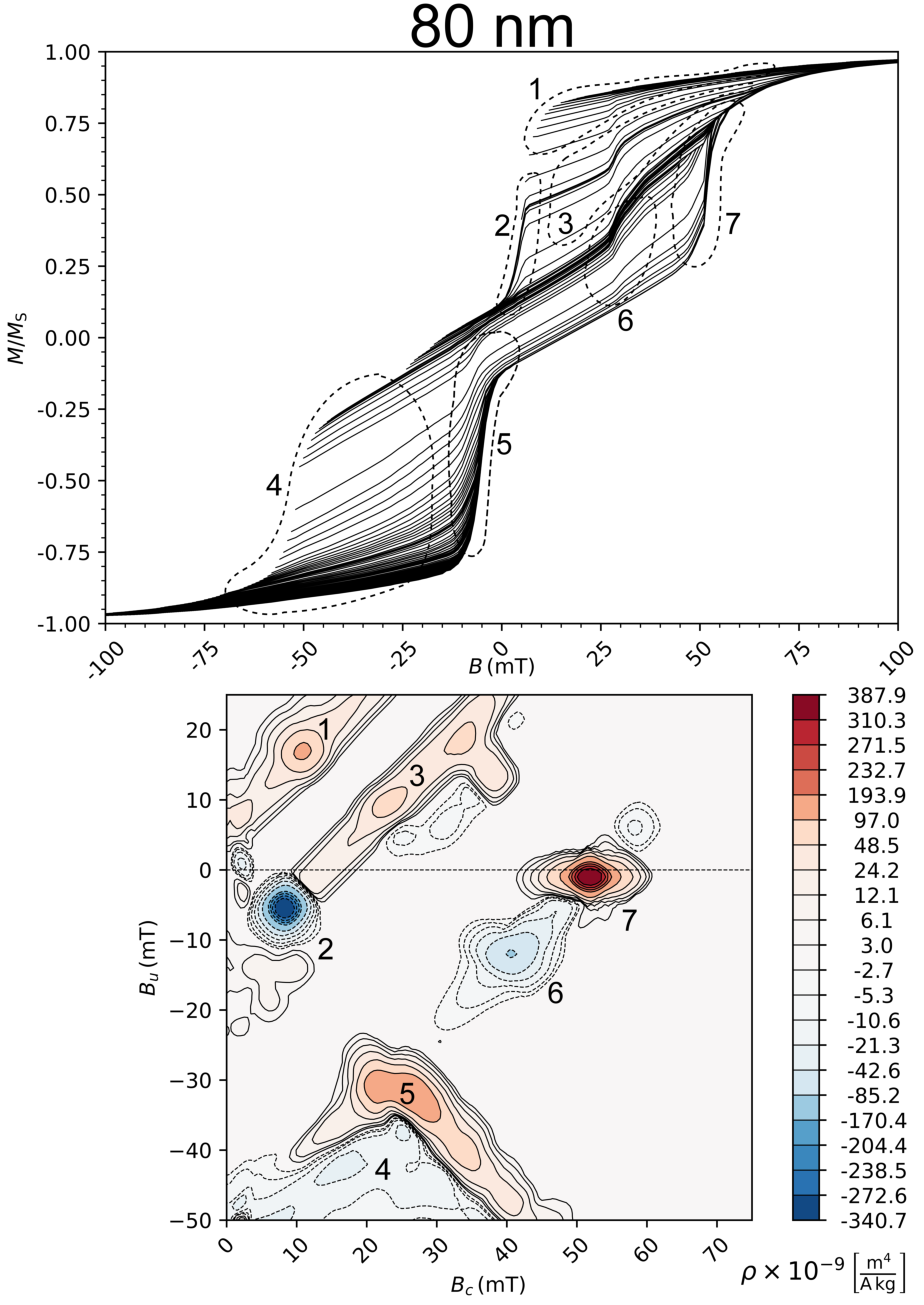
\includegraphics[width=0.9\textwidth]{research-3/figs/FIG_07.pdf}
\caption[FORC diagram and hysteresis curves of 80$\nm$-sized particles]{FORC diagram (SF=4) (bottom) and hysteresis curves (top) for 80$\nm$ particles. Annotations link the FORC diagram responses to the raw hysteresis curves. See text for details. Dashed contour lines on the FORC diagram denote negative $\rho$ values.}
\label{FIG_C4_07}
\end{figure}\par

Particles with hard axes aligned closely with the applied field nucleate hard-aligned vortices at high applied field values (Figs. \ref{FIG_C4_hardaxis}a, \ref{FIG_C4_08}); as the field decreases below $\roughly 12\mT$ these vortices rotate irreversibly to an easy axis alignment (Fig. \ref{FIG_C4_hardaxis}b). As the field is increased on reversal curves with $\roughly 0\mT \leq B_a \leq \roughly 12\mT$ these vortices switch irreversibly back to a hard alignment at $B_b\approx 28 \mT$ to create a local peak at $B_c \approx 12 \mT,\, B_u \approx 16 \mT$ (Fig. \ref{FIG_C4_07}, region 1); this is manifested in the raw hysteresis data by the smoothed discontinuity at $B\approx 28 \mT$ whereas the reversible motion traced by the reversal curves around this region accounts for the tilted, elongated response surrounding the local peak.
\begin{figure}
\centering
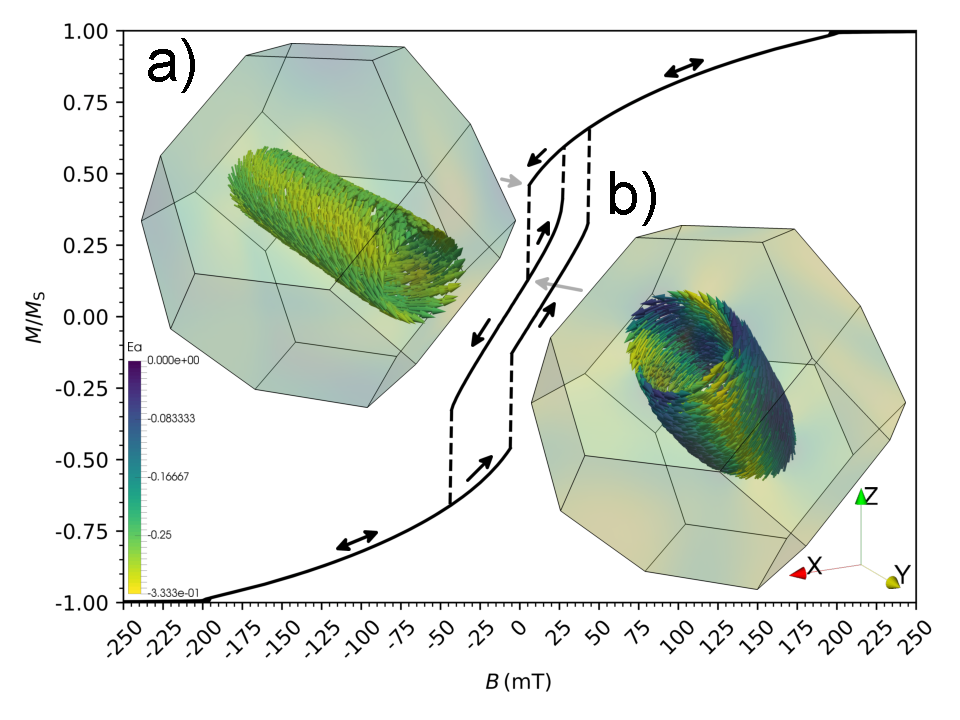
\includegraphics[width=\textwidth]{research-3/figs/BMforcs_080nm_015_edit.pdf}
\caption[Hysteresis of 80$\nm$-sized particle with applied field along a hard axis]{Hysteresis main branch, reversal curves and micromagnetic solutions of 80$\nm$-sized particle with applied field along a hard $<$010$>$ axis. A hard-aligned vortex nucleates at high values of the applied field with a negligible net magnetisation change and therefore negligible contribution to the FORC distribution. The vortex is stable as the field is decreased down to 6$\mT$ (a). Decreasing the field to 5$\mT$ causes the vortex core to rotate irreversibly to an easy $<$111$>$ axis (b). A reversal curve starting at this switching value rotates back to the hard axis alignment when the field is increased to 28$\mT$. The vortex cores are highlighted by their helicity ($m \cdot \nabla \times m$) and coloured according to the anisotropy energy.}
\label{FIG_C4_hardaxis}
\end{figure}\par

During hysteresis, as the remanent state is approached, all particles $\geq 76 \nm$ have nucleated vortices: particles with easy axis alignment close to the applied field directly nucleate an easy-aligned vortex while the rest nucleate vortices initially oriented along hard $<$100$>$ or $<$110$>$ directions (Fig. \ref{FIG_C4_08}b), which rotate irreversibly to an easy axis alignment as the field approaches zero. The latter fraction of particles then undergo irreversible rotations to intermediate positions for $\roughly{-}10\mT \leq B \leq \roughly{-}20\mT$. For FORCs with $\roughly{-}10\mT \leq B_a \leq \roughly{-}20\mT$, these vortices rotate back to the initial easy axis alignment at $B_b\approx 4 \mT$. A combination of these irreversible events creates the lowest negative FORC response (Fig. \ref{FIG_C4_07}, region 2). A further applied field increase to $\roughly 30 \mT$ causes these vortices to switch to the initial hard position from which they nucleated. These events cause the tilted, elongated FORC response (Fig. \ref{FIG_C4_07}, region 3).\par

As the applied field decreases past $\roughly{-}52 \mT$, the vortices of particles with easy axis alignment close to the applied field annihilate (Fig. \ref{FIG_C4_08}). Reversal curves with $\roughly{-}80\mT \leq B_a \leq \roughly{-}52\mT$ trace lower slopes with decreasing $B_a$ due to the combined reversible motion of vortices and single domains; this is the source of the faint negative contribution for $B_u < \roughly 45 \mT$ (Fig. \ref{FIG_C4_07}, region 4). On increasing $B_b$ on these curves, nucleation of easy-aligned vortices occurs at $\roughly{-}5 \mT$ creating the boomerang-shaped response (Fig. \ref{FIG_C4_07}, region 5) that limits the faint negative response in region 4; this corresponds with the smoothed discontinuity in hysteresis curves as the field approaches zero from the left. Increasing the applied field to positive values causes the easy-aligned vortices of particles with hard axes close to the applied field to switch to hard alignments at $\roughly 28 \mT$, creating a negative FORC region (Fig. \ref{FIG_C4_07}, region 6). The distribution peak at region 7 (Fig. \ref{FIG_C4_07}) corresponds to the average annihilation field of the vortices on the reversal paths to positive saturation.
\begin{figure}
\centering
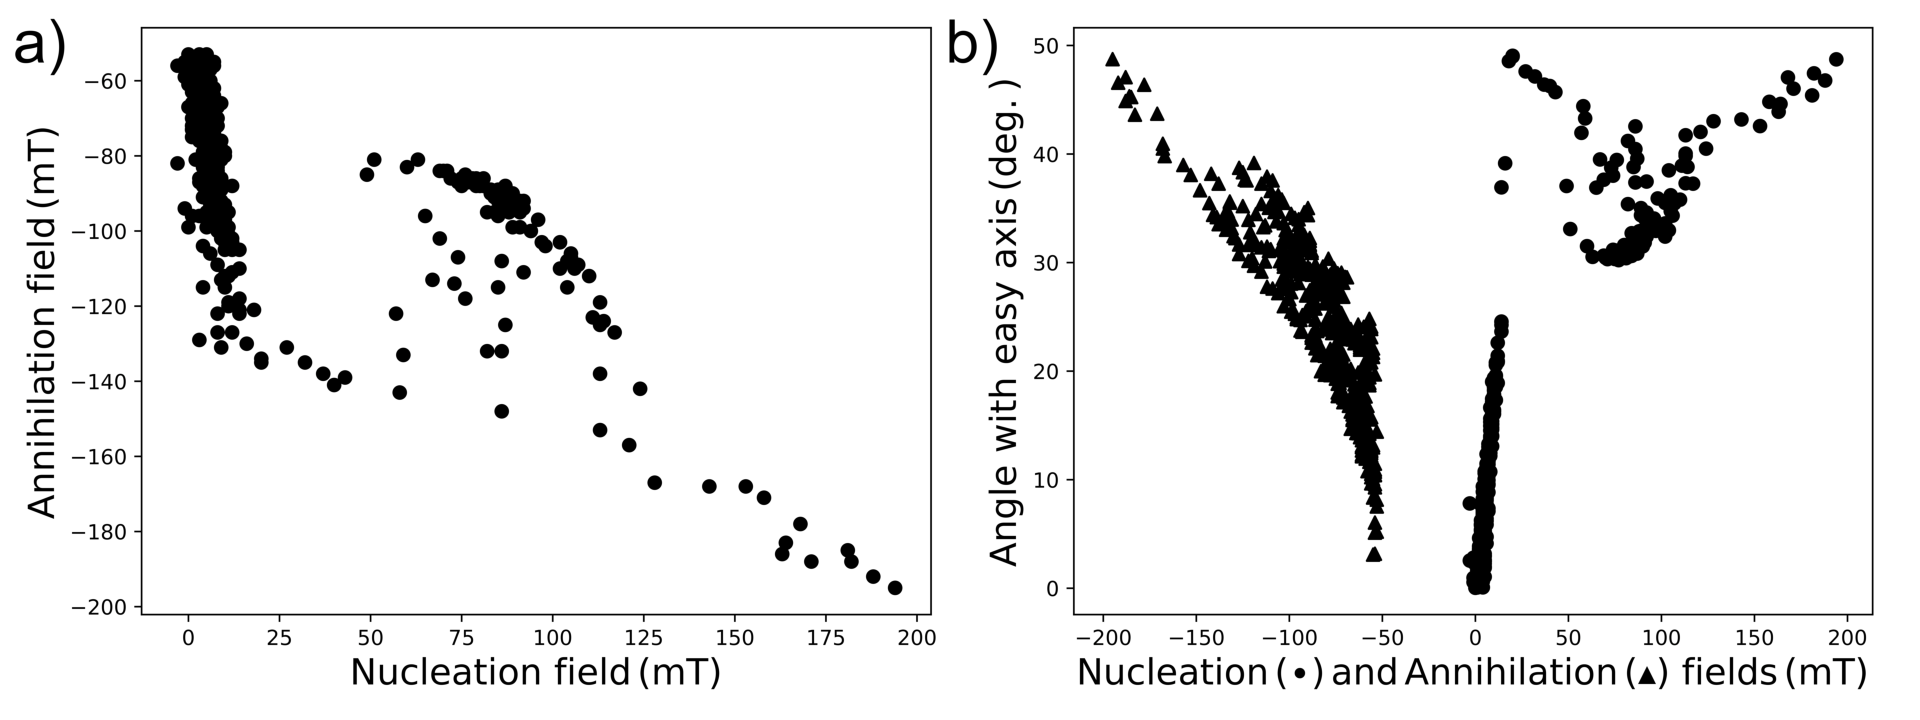
\includegraphics[width=\textwidth]{research-3/figs/FIG_08.pdf}
\caption[Vortex nucleation/annihilation fields]{Vortex nucleation and annihilation fields for the simulated particle ensembles. a) Scatter plot of annihilation field against nucleation field. Three trends are observed depending on whether the nucleated/annihilated vortex has an easy, hard or other alignment. b) Vortex core angle with an easy direction against the nucleation and annihilation fields (circles and triangles, respectively).}
\label{FIG_C4_08}
\end{figure}\par

There is a large spread in the vortex nucleation and annihilation fields (Fig. \ref{FIG_C4_08}). Particles with hard axis alignment close to the applied field nucleate hard-aligned vortices for fields as high as $\roughly 200 \mT$ and annihilate on the opposite side of the particle for equally high (absolute) values. However, these nucleation and annihilation events make a negligible contribution to the FORC diagram because the change in magnetisation of a particle nucleating/annihilating a hard-aligned vortex from/to a SD state can be as low as $1 \%$.\par

%-----------------------------------------------------
\section{Discussion}
Comparison of results for micromagnetic simulations presented here with the coherently rotating dipole model of \citet{ValdezGrijalva2017} indicates excellent agreement (Fig. \ref{FIG_C4_02}). This confirms the accuracy of our model using only 500 random field orientations instead of field orientations on a regular grid, which requires a high density of field orientations near the poles of the sphere. A FORC diagram for SD coherently rotating particles has the same general features as those obtained for weakly interacting SD particles with cubic MCA by \citet{Harrison2014}, i.e., a positive ridge along the $B_c$ axis, slightly offset toward $B_u<0$ values and a tilted, negative ridge on the lower half of the FORC plane. For these ensembles, the horizontal spread along the $B_c$ axis corresponds to the density of switching fields of the differently oriented particles and the FORC distribution peak position corresponds directly to the ensemble coercivity. The negative ridge is indicative of intermediate states along the hysteresis curve and, therefore, of SD particles with non-uniaxial (in this case cubic) MCA \citep{ValdezGrijalva2017}; this type of FORC response has been identified in simulations for magnetite \citep{Harrison2014} and hematite \citep{Harrison2017}, and is potentially unique to non-interacting to weakly interacting SD particles with cubic or other non-uniaxial MCA. Experimental data from the Vulcan iron formation (Michigan, USA) \citep{Laird2017} shows very similar FORC diagram patterns for a mixture of SD magnetite and hematite (Fig. \ref{FIG_C4_Laird2017}).
\begin{figure}
\centering
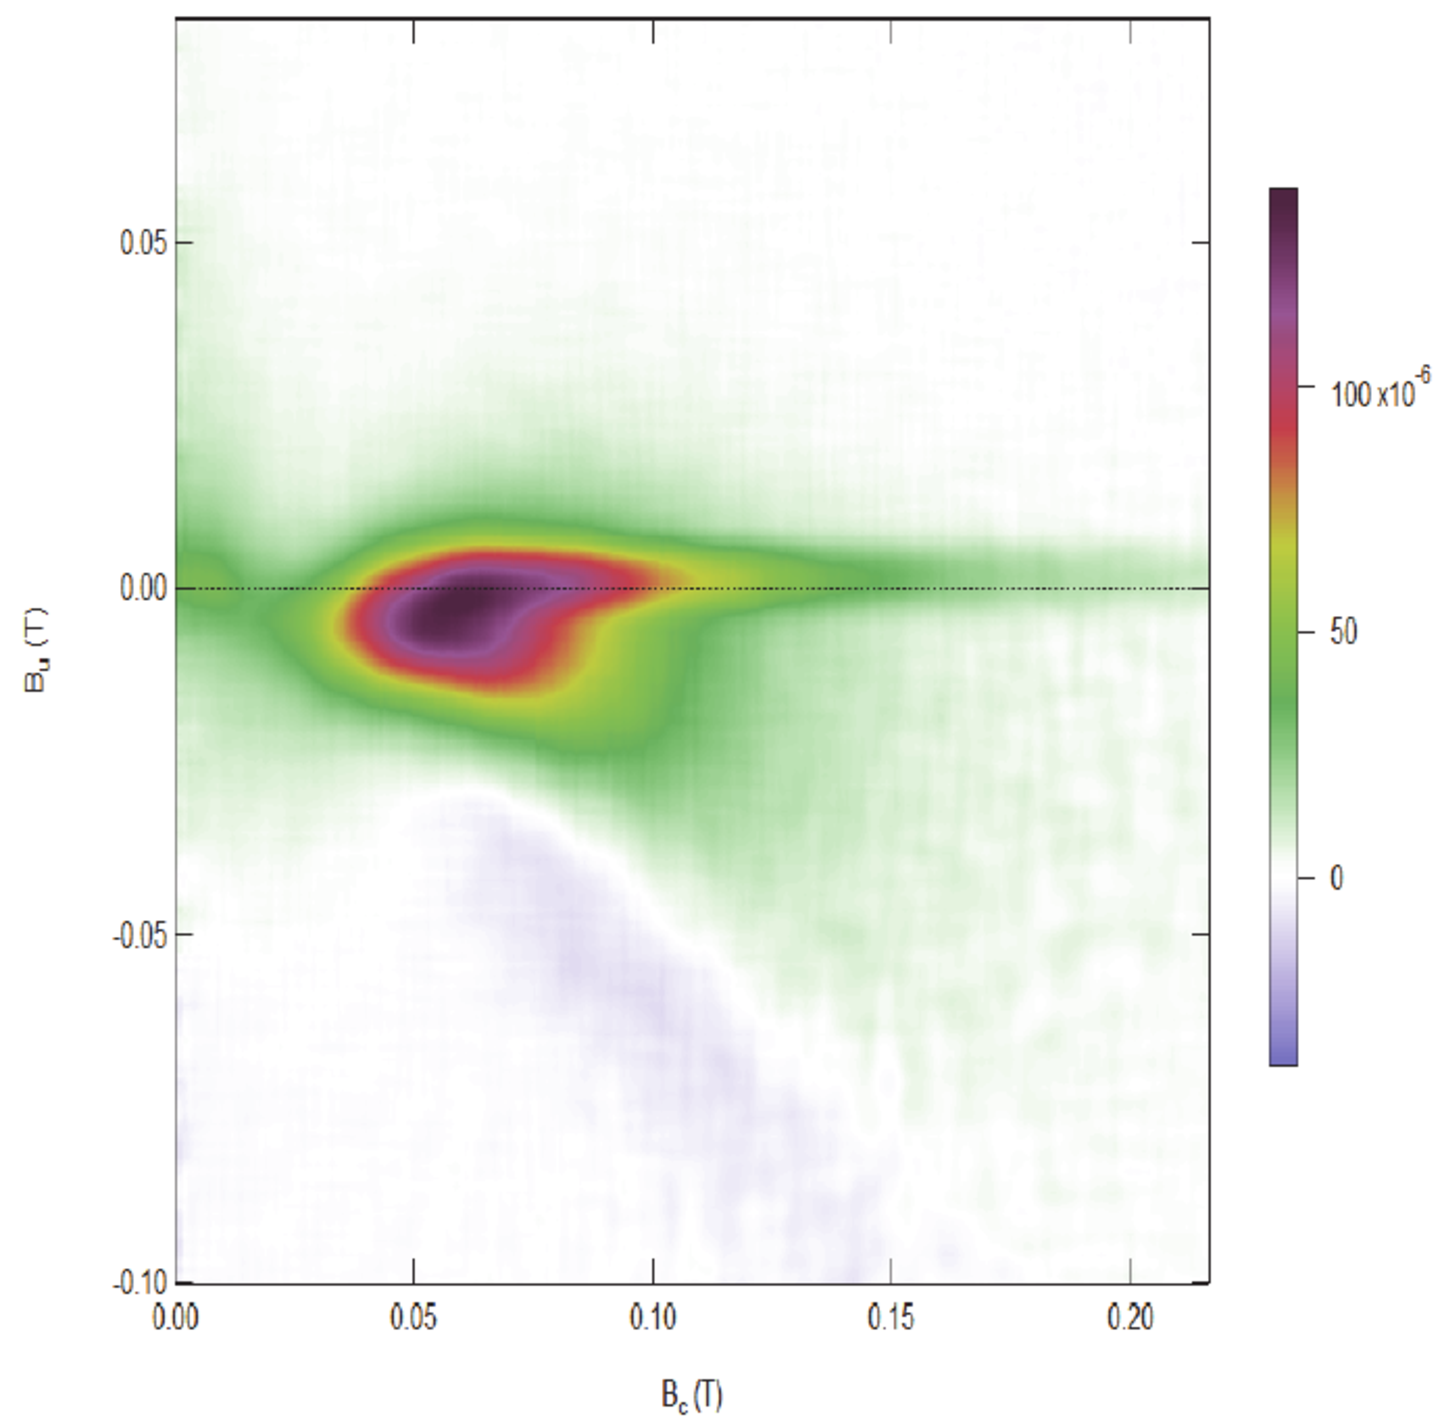
\includegraphics[width=0.6\textwidth]{research-3/figs/Laird2017_thesis.pdf}
\caption[FORC diagram of a SD magnetite and hematite sample]{FORC diagram (SF=6) of a SD magnetite- and hematite-dominated sample from the Vulcan iron formation (Michigan, USA). (From \citet{Laird2017}, reproduced with permission from the author).}
\label{FIG_C4_Laird2017}
\end{figure}\par

The coercivities obtained here are considerably lower than the commonly accepted value for natural greigites of $\roughly 60\mT$. This discrepancy could be explained by shape anisotropy effects: if the greigite grains are slightly elongated, shape anisotropy can increase the coercive fields, therefore the FORC distribution would shift towards higher $B_c$ values. The effect of shape anisotropy would also remove the tilted, negative ridge as no intermediate states along the hysteresis main branch would exist. SD greigite is commonly diagnosed from concentric FORC distributions centered at $B_c \approx 60\mT$ \citep{Roberts2011} without the tilted, negative ridge. Another possibility is for magnetostriction effects to induce a uniaxial anisotropy and increase the coercivities. However, the magnetostrictive properties of greigite are poorly understood.\par

Whereas the pure SD signal produces a tight, boomerang-shaped FORC distribution (Fig. \ref{FIG_C4_02}), increasing particle size introduces SV structures that fragment this pattern. The FORC distribution peak is moved toward higher $B_c$ values along the $B_u=0$ axis. Paradoxically, as this occurs, the bulk coercivity of the ensembles decreases (Fig. \ref{FIG_C4_05}). This paradox has been observed previously by \citet{Dumas2007} in synthetic size-controlled samples of sub-100$\nm$ Fe dots (Fig. \ref{FIG_C4_Dumas2007}).
\begin{figure}
\centering
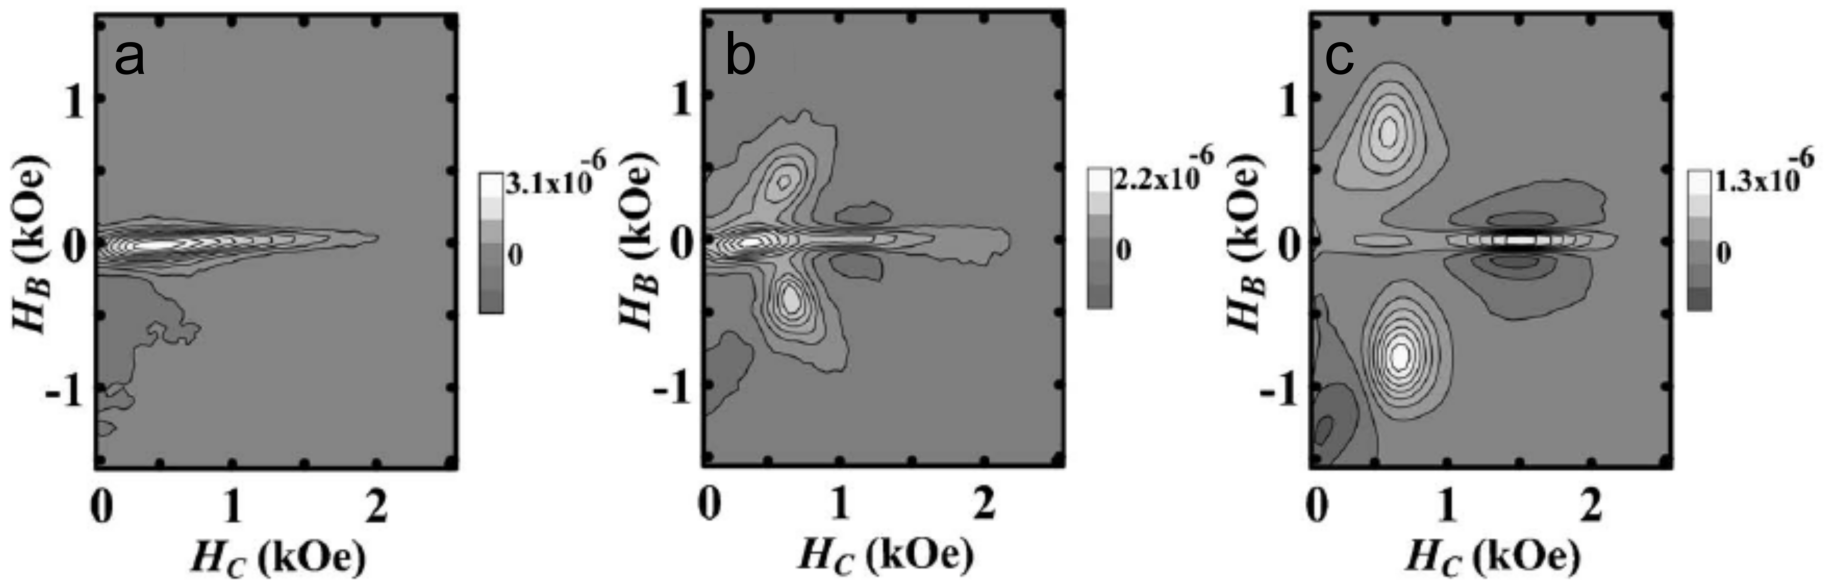
\includegraphics[width=\textwidth]{research-3/figs/Dumas2007_edit.pdf}
\caption[FORC diagram of a synthetic Fe dot array]{FORC diagrams for a weakly interacting 2D array of Fe dots fabricated using a nanoporous alumina shadow mask technique in conjuction with electron beam evaporation. a) The array with the smallest (52$\nm$) particles shows SD properties. b) The array with 58$\nm$ particles shows SD and PSD properties. c) The array with the largest particles (67$\nm$) shows purely PSD properties. (From \citet{Dumas2007}, reproduced with permission from the author).}
\label{FIG_C4_Dumas2007}
\end{figure}\par

Fragmentation of the FORC diagram for non-uniformly magnetised particles has been observed in experimental studies \citep{Pike1999B,Dumas2007,Roberts2017,Zhao2017} (Fig. \ref{FIG_C4_Dumas2007}) and in numerical models \citep{Carvallo2003,Roberts2017}; however, these studies did not include random field orientation distributions. The trend is, nevertheless, clear and is representative of the complex self-interactions brought about by nonuniform structures and multiple vortex nucleation/annihilation fields \citep{Pike1999B}. It is difficult to compare our results to the FORC signals measured by \citet{Muxworthy2006B} and \citet{Krasa2011} for synthetic patterned magnetite because many of their FORC diagrams appear to have smoothed the subtle features observed here, which raises questions about the integrity of these samples (e.g., crystallinity) or the adequateness of the FORC measurement density for these samples. However, a general trend is recognised in the elongation of the FORC diagram contours in the direction of a negative angle diagonal from the $B_u=0$ axis (Fig. \ref{FIG_C4_Muxworthy2006B}) probably related to region 5 in Fig. \ref{FIG_C4_07}. FORC diagrams for coarse-grained synthetic greigite samples by \citet{Roberts2011} also show this type of elongations as well as a negative ridge (Fig. \ref{FIG_C4_Roberts2011}) probably caused by a fraction of SD particles.
\begin{figure}
\centering
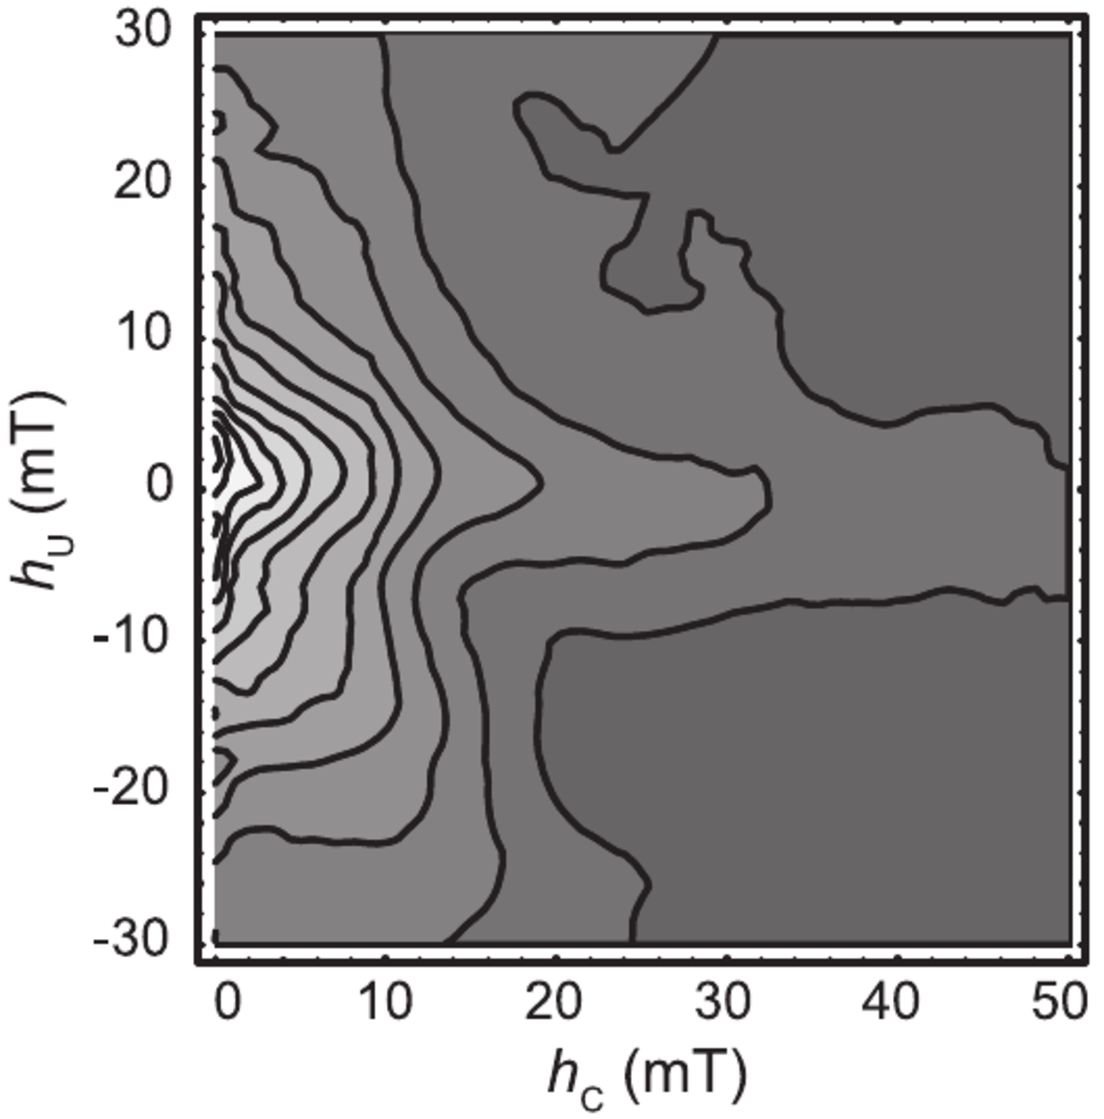
\includegraphics[width=0.4\textwidth]{research-3/figs/Muxworthy2006B.pdf}
\caption[FORC diagram of a synthetic magnetite 2D array]{FORC diagram (SF=4) for a weakly interacting 2D array of synthetic magnetite produced by electron beam lithography. Applied field along the elongation of the grains. (From \citet{Muxworthy2006B}, reproduced with permission from the author).}
\label{FIG_C4_Muxworthy2006B}
\end{figure}\par

\citet{Pike1999B} obtained asymmetric nucleation and annihilation fields of magnetic vortices in nano-patterned Co dots; our models agree with this finding (Fig. \ref{FIG_C4_08}). However, \citet{Pike1999B} studied elongated disc-like particles where the vortex cores were always perpendicular to the particle plane that mostly underwent reversible motion from nucleation to annihilation as they traversed the particle. In this study, we demonstrate that different features on SV FORC diagrams are due to a variety of vortex nucleation and annihilation events, which depend on particle alignment with respect to the applied field and on the presence of distinctly different vortex states, i.e., the vortex energies and stabilities depend on their alignment within the crystalline structure \citep{ValdezGrijalva2017B}.
\begin{figure}
\centering
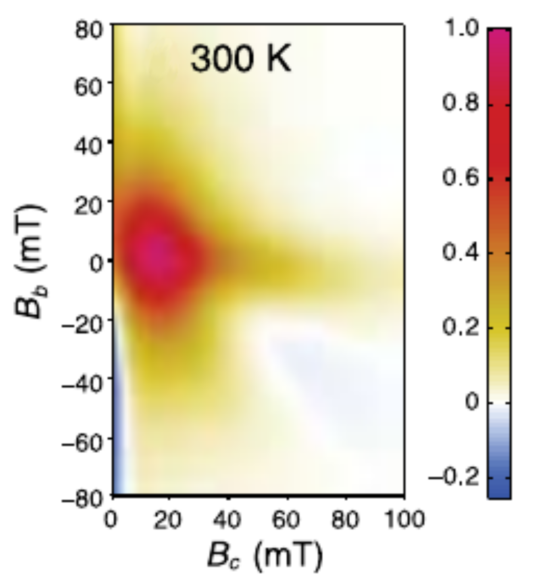
\includegraphics[width=0.4\textwidth]{research-3/figs/Roberts2011_edit.pdf}
\caption[FORC diagram of a synthetic coarse-grained greigite sample]{FORC diagram (SF=3) for a synthetic coarse-grained greigite sample of predominantly PSD particles. (From \citet{Roberts2011}, reproduced with permission from the author).}
\label{FIG_C4_Roberts2011}
\end{figure}\par

FORC diagrams were averaged for simulations between 30 and 80$\nm$ (Fig. \ref{FIG_C4_09}a) and between 60 and 80$\nm$ (Fig. \ref{FIG_C4_09}b). That is, the particle size distributions are uniform (flat) for these averaged FORC diagrams. The FORC diagram in Fig. \ref{FIG_C4_09}a has a boomerang-shaped distribution surrounded by a variety of more complex responses. This pattern shows some similarities to the patterns observed by \citet{Dumas2007} for samples that included both SD and SV particles. The FORC distribution peak position coincides with the ensemble coercivity, while still having a response corresponding to the annihilation field of easy-aligned vortices.
\begin{figure}
\centering
\includegraphics[width=\textwidth]{research-3/figs/FIG_09.pdf}
\caption[Averaged-over-size FORC diagrams and raw hysteresis curves]{Averaged FORC diagrams (SF=4) (top) for multiple particle sizes and corresponding raw hysteresis curves (bottom). Uniform size distributions are used for particles a) $30\nm \leq d \leq 80\nm$ and b) $60\nm \leq d \leq 80\nm$. Dashed contour lines denote negative $\rho$ values.}
\label{FIG_C4_09}
\end{figure}\par

Both diagrams in Fig. \ref{FIG_C4_09} have a significant spread in the positive $B_u$ region. This effect is purely due to domain state, not magnetostatic interactions. The main peak for the averaged SV-dominant diagram (Fig. \ref{FIG_C4_09}b) occurs along the $B_u=0$ axis at $B_c\approx 52\mT$, which indicates a disconnect with the bulk coercivity of the ensemble ($B_\text{C}\approx 16\mT$). This is a departure from the usual interpretation of FORC diagrams, i.e., that the FORC diagram provides a map of the coercivity distribution. This interpretation holds for SD coherently rotating grains, where the peak response coincides with the value of the ensemble coercivity. It does not hold, however, for SV grains because their coercivity decreases with size while the position of the maximum moves toward higher $B_c$ values. Instead, for SV grains the FORC distribution peak, and most FORC features, should be interpreted as due to vortex nucleation/annihilation fields and their irreversible motions.\par
%-----------------------------------------------------

\section{Conclusion}
A micromagnetic FEM/BEM was employed to calculate FORC distributions for non-interacting ensembles of greigite across a size range that spans the SD to SV threshold. 500 random orientations from a uniform distribution over a sector of the unit sphere were used for each particle size. This choice was found to be in excellent agreement with previous calculations for SD greigite \citep{ValdezGrijalva2017}.\par

FORC diagrams are found to be extremely sensitive to the domain state of the simulated particles. When even a small fraction of particles starts to nucleate vortices, e.g., $d\approx$50$\nm$, this is reflected in the FORC diagram (Fig. \ref{FIG_C4_03}a compared to Fig. \ref{FIG_C4_02}). The same cannot be said of the Day plot (Fig. \ref{FIG_C4_05}a). Anomalous behaviour for particles sized 62 to 72$\nm$, with coercivity increasing with size was found; these particles plot in an unexpected region of the Day plot. The anomaly disappears for particles $>72\nm$, and when $d \geq 76\nm$ they have much lower $M_\text{RS}/M_\text{S}$ and higher $B_\text{CR}/B_\text{C}$ values.\par

Detailed FORC analysis and micromagnetic solutions for $d=80\nm$ particles reveals the meaning of the FORC diagram for SV ensembles as a map of vortex nucleation/annihilation fields. Interpretation of FORC diagrams as a coercivity distribution does not apply to SV systems (see \citet{Pike1999B,Roberts2017}). Recognition that the remanence in palaeomagnetic studies is often carried by vortex state particles should help users of FORC diagrams to avoid misinterpretation of vertical spread in FORC diagrams, just as it is recognised that vertical spread in MD particles is due to domain wall interactions within particles \citep{Pike2001}. For SD particles, the typical interpretation of the peak position coinciding with the coercivity of the sample holds; however, for SV-dominated samples, the position of the peak occurs at a value much higher than the bulk coercivity of the sample.\par
%-----------------------------------------------------
%\renewcommand\bibname{{References}}
%\bibliographystyle{elsarticle-harv}
%\bibliography{references}


